\chapter{Module Role and Scope}

\section*{Role of the Coffee Chain ERP Module}

The Coffee Chain ERP module is designed to consolidate multiple business functions into a single, integrated platform. Its role is to streamline operations, improve data visibility, and provide actionable insights for decision-makers across the coffee outlet network. Specifically, the module serves the following purposes:

\begin{itemize}
    \item \textbf{Outlet Management:} Maintain records of outlet details such as name, location, assigned manager, and regional manager. This ensures consistent operational oversight across all outlets.
    \item \textbf{Sales Management:} Capture daily sales transactions, link sales with menu products, track revenue per outlet, and generate performance reports.
    \item \textbf{CRM Integration:} Manage customer leads, track interactions, and associate them with sales outcomes to enhance customer relationship management.
    \item \textbf{Menu Integration:} Administer coffee menu items, categories, and pricing, with automatic synchronization to the Sales module for real-time ordering.
    \item \textbf{Data Consolidation and Analytics:} Centralize information from multiple outlets for analysis, reporting, and decision-making.
\end{itemize}

\vspace{1em}

\section*{Scope}

The scope of the Coffee Chain ERP module defines its boundaries and functionalities:

\begin{itemize}
    \item Covers all active coffee outlets within the chain.
    \item Includes management of all menu items, product categories, and pricing.
    \item Captures daily sales transactions and integrates them with menu and CRM data.
    \item Provides real-time dashboards and reports for outlet managers and regional managers.
    \item Supports operational decision-making based on consolidated performance metrics.
    \item Excludes loyalty and reward management in the current version.
    \item Does not include outlet capacity tracking; operational staffing and space management are outside the current module scope.
\end{itemize}

\vspace{1em}

\section*{Stakeholders and KPIs}

The primary stakeholders and associated KPIs are outlined below:

\begin{itemize}
    \item \textbf{Outlet Managers:} Monitor outlet efficiency, daily revenue, and sales performance.  
          \textit{KPIs: revenue per outlet, sales per product, top-selling items.}
    \item \textbf{Regional Managers:} Compare performance across outlets within their region.  
          \textit{KPIs: total revenue, average sales per outlet, regional growth trends.}
    \item \textbf{Employees:} Ensure accurate data entry for sales, products, and customer interactions.  
          \textit{KPIs: transaction accuracy, product update consistency.}
    \item \textbf{Management and Decision-makers:} Access consolidated insights for strategic planning and operational improvements.  
          \textit{KPIs: lead conversion rate, overall revenue, sales growth trends.}
\end{itemize}

\vspace{1em}

\section*{Module Context Diagram (C1)}

The C1-Level Context Diagram illustrates the Coffee Chain ERP module, showing its interactions with key stakeholders, submodules (Outlet, Sales, Menu, CRM), and the flow of information between them.

\begin{figure}[H]
\centering
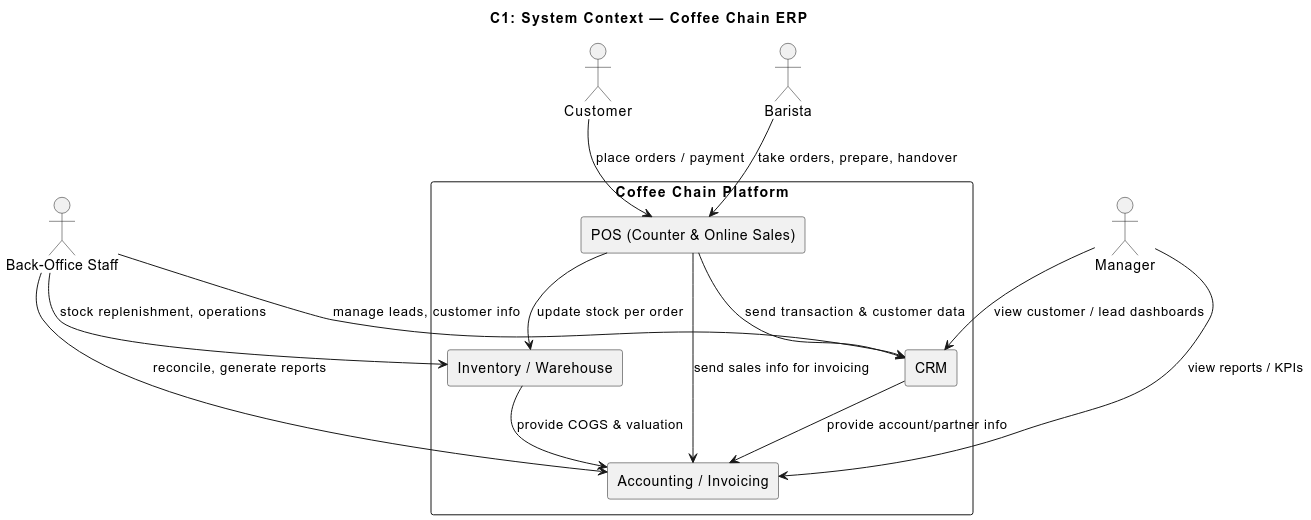
\includegraphics[width=0.9\textwidth,keepaspectratio]{diagrams/context.png}
\caption{C1-Level Context Diagram of Coffee Chain ERP}
\end{figure}

The diagram highlights how outlet data, sales transactions, menu updates, and CRM leads flow into the ERP system. Management and regional managers receive consolidated reports and insights. Each module interacts seamlessly to reduce manual work, ensure real-time synchronization, and improve decision-making.

\vspace{1em}

\section*{Insights}

\begin{itemize}
    \item The Coffee Chain ERP module centralizes multiple business functions, reducing operational fragmentation across outlets.
    \item Integration between Outlet, Sales, Menu, and CRM ensures real-time data synchronization, minimizing errors and manual updates.
    \item Consolidated dashboards and reporting empower managers and regional managers to make informed operational and strategic decisions.
    \item Linking menu items directly to sales products automates pricing updates and sales tracking, improving accuracy and efficiency.
    \item CRM integration enhances customer relationship management, allowing the business to track leads, improve engagement, and monitor conversion rates.
    \item The module provides a foundation for future expansions such as loyalty programs, outlet capacity tracking, or advanced analytics.
    \item By visualizing the system through the C1-Level Context Diagram, stakeholders can clearly understand interactions, responsibilities, and information flows.
    \item Overall, the ERP module streamlines multi-outlet operations, increases transparency, and strengthens decision-making capabilities across the coffee chain.
\end{itemize}
